\chapter{Copy Control} \label{CHAP:COPYCTL}

Since there are no slides and the copy control ex. sheet is about processes (i.e., control overhead chapter -.-, we rely on the book for this one).

\textit{Short description:} Copy control focuses on removing the obvious waste (P1) of copying when unnecessary, i.e, not imposed by hardware. Some copies such as those when an adapter receives data and forwards it to the kernel are simply necessary.

A mapping from principles to problems and solutions is given in the following table:

\begin{tabular}{|c|p{8cm}|c|}
\hline 
Number & Principle & Used in \\ 
\hline 
P13 & Memory location (on adaptor) as degree of freedom) & Afterburner \\ 
\hline 
P2b & Lazy copying using copy-on-write & Mach \\ 
\hline 
P11a and P7 & Cache VM mappings per path, Uniform fbuf space across processes & Solaris fbufs \\ 
\hline 
P10 & Pass buffer name and offset in packet & RDMA systems \\ 
\hline 
P4 & VM mapping to avoid copies in cache and apllication & Flash \\ 
\hline 
P11a & Cache VM mappings per path, Buffer sequence numbers enable checksum caching & Flash-lite \\ 
\hline 
P6 & New system call that splices I/O & Sendfile() \\ 
\hline 
P1 & Avoid repeated memory access across manipulations & ILP \\ 
\hline 
P13 & Layout code to minimize i-cache misses & x-kernel \\ 
\hline 
P13 & Layer processing order as degree of freedom & LDRP \\ 
\hline 
\end{tabular} 

\section{Why remove extra copies?}

This is kind of obvious:

\begin{itemize}
    \item It uses memory resources
    \item Takes time
\end{itemize}

Main hardware players in a server:

\begin{itemize}
    \item CPU
    \item Memory BUS
    \item I/O Bus
    \item Disk
    \item Network adaptor
\end{itemize}

Example of redundant copies in a Webserver:

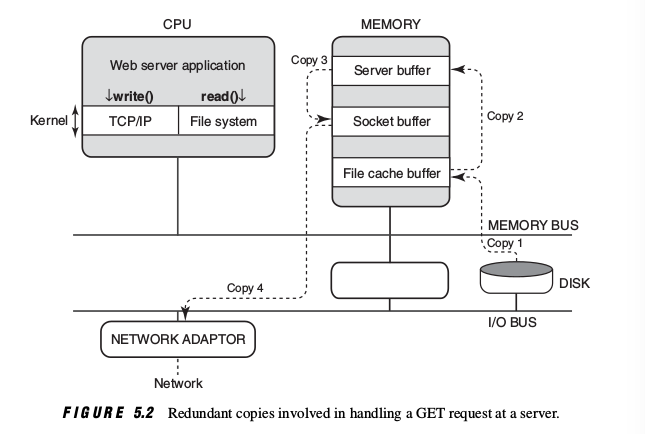
\includegraphics[width=.7\textwidth]{images/chap5/Redundant_copies}

In this example we can observe as much as 4 copies for one task.

\section{Reducing copying via local restructuring}

\subsection{Exploiting adaptor memory:} 

Memory can be located anywhere on the bus in a memory-mapped architecture. Usually, kernel memory is on memory subsystem, but there is no reason that part of it can't be on kernel (except for some security concerns -.-).

In our example, the socket buffer would now lie directly on the network adaptor and the data would be copied from the server buffer onto the socket buffer. The example in the book ignores disk-to-memory copies, which would be necessary additionally.

\textbf{Problems of this approach:}

\begin{itemize}
\item Network adaptor needs lots of memory to provide such functionality
\item Corrupted data may be written to application buffers in some cases
\item This approach may result in delayed acknowledgments (not discussed in the book but mentioned)
\end{itemize}

\subsection{Using Copy-on-Write}

We discussed this in the lecture. Copy-on-write means that an application can use memory used by another process in kernel space, as long as it doesn't write to it. When it writes data to the buffer it has to finally be copied, which may not always be the case, hence it is a good improvement.

In this case, unlike the previous solution, we want to get rid of the copy from user space to kernel space, i.e. server buffer socket buffer. (server in terms of webserver). 

\textbf{Idea:}

\begin{itemize}
    \item Replicate virtual page in memory at low cost
    \item Make the copy point to the original physical page
    \item If owner of data modifies data, OS will notice and generate two separate copies
\end{itemize}

Performance is gained under the assumption that the application does not modify it's buffer while the kernel works with it.

In our example, the buffer is represented as Server + Socket buffer in one block.

\subsection{Fbufs: Optimizing Page Remapping}

When assigning a new page in the pagemap, simply pointing to the data is not sufficient if it's owned by another page (which is mostly the case when we talk about copies).

Additional pieces of overhead that we need to take care of when copying:

\begin{itemize}
    \item Multiple-level page tables: Systems have multiple levels, thus multiple levels of pages may have to be changed.
    \item Acquiring locks and modifying page table entries: Page tables are shared resources, need protection
    \item Flushing translation look-aside buffers: Page Table Mappings are usually cache in TLB. New VP $\rightarrow$ TLB entries must be found and flushed
    \item Alloc. VM in dest. domain: Computation needed to find free page
    \item Locking the corresponding pages: Pages can be swapped to disk to make place, prevention needs locks and additional overhead.
\end{itemize}

\textbf{FBUFS Idea:} Buffer will be reused, OS can precompute page mapping information, avoids computational overhead during data transfer.

Simple way to implement is using \textit{shared memory}. Map pages $P1,\dots ,P_N$ into virtual memory tables of kernel and applications: \textbf{Bad idea!} Security violations and fault-isolation violations..

More secure: Reserve (lazy) mapped shared pages for each application-to-kernel transfer and vice versa. I.e., one set of buffer pages for FTP, one for HTTP, one for SSH and so on. OSs define multiple security domains, fbuf designers call paths sequences of security domains.

\textbf{Implementation:} Take physical pages $P1, \dots , P_k$, premap to page tables of ethernet driver, the network stack and the server (application). Reserving pages for every path can be wasteful, due to burstiness of networking, rather lazily establish mappings when paths are busy.

Network adaptor needs to quickly find which path a packet takes $\rightarrow$ \textit{early demultiplexing} (chapter 8). The adaptor has a list of free buffers, which it writes the packet to.

Additionally, designers of fbufs insisted on having it mapped onto the same VP in all applications to not have to search for it (P7, unnecessary generality).

\textit{Note:} I think more detail is unnecessary, this is enough detail. ATM the design only allows one writer and multiple readers, the book has a solution for that too.

\subsection{Transparently emulating copy semantics}

Goal: Realize (some) ideas of \textbf{fbufs}, without changing the underlying systems API. The system by Brustoloni and Steenkiste called \textbf{TCOW} (transient copy on write) should solve this problem. (Note, there has not been experimental confirmation of whether this works, as far as the book author is concerned)

\textbf{Idea:} Standard API requires possibility for applications to alloc. dealloc. buffer to kernel (fbuf makes this illegal). OS must deal with application writes and deallocations during time where kernel uses the buffer. \textit{Genie} system solves it as follows:

\textbf{Handle write threats:} \begin{itemize}
    \item When application writes, buffer is marked as read only
    \item Virtual memory fault manager is invoked
    \item If OS preserves copy-semantics, no error occurs
    \item Genie hence modifies error handler:
    \item First: For each page/buffer, keep track if outstanding sends exist (network sends)
    \item Second: Error handler makes copy of page for the application, thus preserving standard copy-semantics
    \item This technique is called \textbf{TCOW}
\end{itemize}

\textbf{Handle deallocate threats}: Normally, process exists to maintain deallocated pages in free list. Hence, daemon can also be modified to not deallocate if page is still used for sending.

In both cases, instances of \textbf{P3b}, shift comp. in space is applied, moving logic to error handler and page deallocator.

\section{Avoid copies using remote DMA}

We only talked shortly about DMA (Direct Memory Access). The idea is to let a piece of hardware directly use a buffer as if it was it's own physical memory. Workload can be taken from the CPU, which may have to chop a huge file or large packet into fragments. Instead the hardware device can write out the chunks and the application can directly use them.

\textbf{RDMA} is the idea of doing \textbf{DMA} over the network, i.e., data is transferred between two computers memories without per-packet mediation between the two CPUs. Two problems occur:

\begin{enumerate}
\item Where is received being placed?
\item Security maintenance? Just think what rogue packets with direct memory access could do ...
\end{enumerate}

\subsection{Avoid copies in a cluster}

In server clusters, for instance webservers, the need for \textbf{RDMA} may arise as data may have to be efficiently copied within the clusters servers. \textbf{VAX} Clusters, a 30 year old product from \textit{Digital Equipment Corp.} (DEC) implemented the idea of RDMA.

\textbf{Problems:} \begin{itemize}
    \item Pages need to be mapped. If Page 1,2,3 arrive in order 1,3,2 and are stored in 1,2,3 the order is broken.
    \item Remapping of large files is expensive.
\end{itemize}

\textbf{Idea for VAX:} Destination app. locks a number of physical pages. Logical view is buffer of consecutive logical pages. Sender now sends information within protocol header (buffer pos., offset..).

\subsection{Modern-Day Incarnations of RDMA}

Vax Clusters are early Storage Area Networks (SAN). Other newer technolgies include \textit{Fiber Channel}, \textit{Infiniband} and \textit{iSCSI}.

\section{Broadening to File Systems}

The last section for copy-control, as I think that we've talked about file copying and file systems as well.
The previous improvements were made to get rid of copies between applications and the network while sending data.

\subsection{Shared Memory} Unix provides system call \texttt{mmap()} that maps a file to virtual memory and other OSs provide similar functions. In theory, when mapped, it's as if a cached copy is in memory (redundant because file system also cache files). Using virtual memory, the file is only a set of mappings, and applications, file server cache and so on, can gain access to pages for the file.

\subsection{IO-Lite: Unified view of buffering}

Using \texttt{mmap()}, copies of dynamically created content are not optimized. Processes that create dynamic content, send it to the server process over a \textbf{pipe}. Also, haven't done anything against TCP checksums, although if the same file is sent over and over again it stays the same.

\textbf{IO-Lite:} "Intellectual descendant of \textbf{fbufs}" . \textbf{fbufs} can't be combined with \texttt{mmap()}, unlike \textbf{TCOW}. Also IO-Lite has Unix implementation, \textbf{fbufs} do not.

Other than that, ideas are from \textbf{fbufs}:

\begin{itemize}
    \item Read-only immutable buffers (IO slices)
    \item Useage of composite buffers (aggregates)
    \item Lazily created cache of buffers for a path (I/O stream)
\end{itemize}

This image should help visualize the underlying architecture:

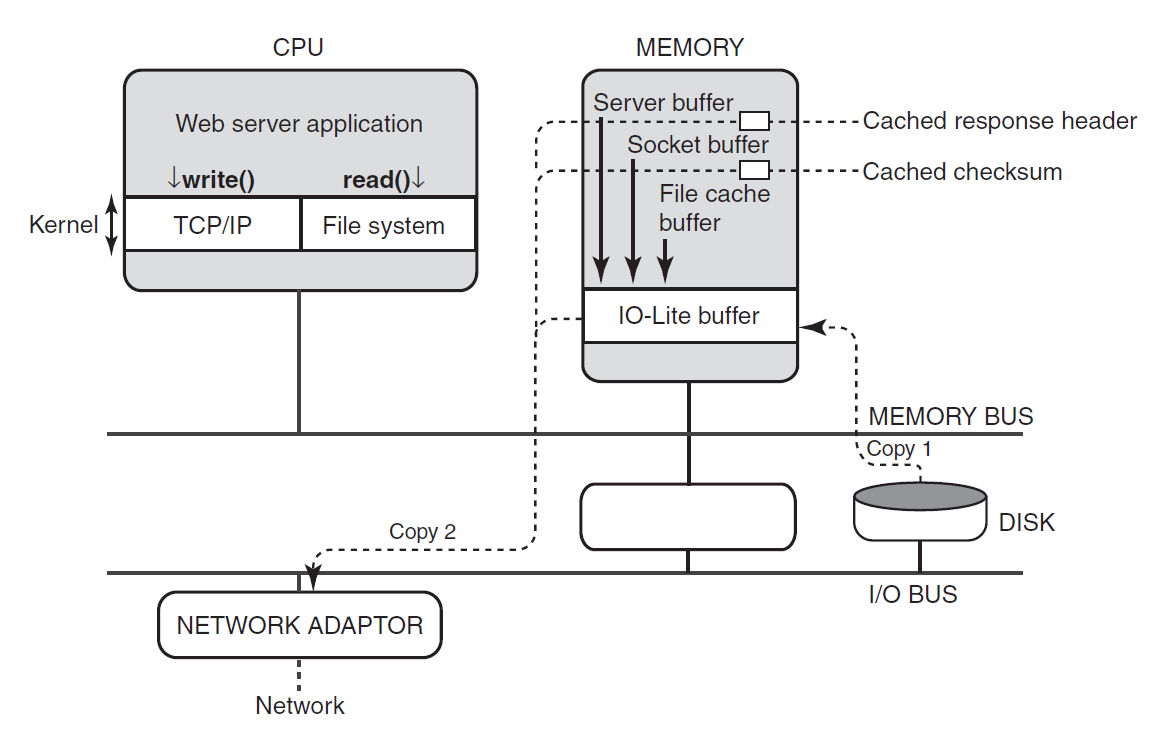
\includegraphics[width=\textwidth]{images/chap5/io_lite}

\textbf{Problems with file system integration:} 

\begin{itemize}
    \item Complex sharing patterns (application, network stack, file system all may point to buffer)
    \item Page can be VM Page and also File Page, hence complex replacement policy needed (standard page replacement and file cache replacement)
    \item Going over an OS (Unix) requires clean way of integration without major changes to the underlying OS
\end{itemize}

The graphic shows the base idea, I don't think we need to know more detail.

\subsection{Avoid file system copies via I/O splicing}

\textbf{IO-Splicing} is used to get rid of all copies we've seen before. Basically, the data goes directly from the file cache buffer to the network adaptor without any intermediary steps. Systems probide calls such as \texttt{sendfile()}, which does exactly that.

















